\documentclass[11pt]{article}
\usepackage[margin=1.1in]{geometry}
\usepackage{amsmath,amssymb}
\usepackage{graphicx}
\usepackage{booktabs}
\usepackage[hidelinks]{hyperref}
\usepackage{microtype}
\graphicspath{{figures/}}
\setlength{\parskip}{2pt}

\title{The Lexical Seam: A Two-Population Account of Word Frequencies that Measures, Explains, and Predicts the Zipf--Mandelbrot Law}
\author{Grigori Karapetyan\\ \small Independent researcher; Nexus Computers LLC; Burbank, CA, USA}
\date{Draft v6.1 --- July 23, 2026}
\begin{document}\maketitle
\begin{abstract}
The Zipf--Mandelbrot (ZM) law, $f(r) \propto (r+c)^{-b}$, has described word rank--frequency distributions for seventy years while leaving unexplained both its systematic apex residual and the behaviour of its parameters. We characterize both through a single object: the \emph{lexical seam}, the boundary region where a small high-usage vocabulary meets the broad remainder of the lexicon. A parameter-free symbolic search shows the residual is reproducible on 25/25 English corpora while its winning symbolic label is an artifact of the scoring objective; identity ablations and two non-linguistic controls locate the residual in the crossing of two word populations. A smooth two-regime model absorbs the residual completely (helpful post-fit corrections on 0/25 corpora, versus 19/25 for the strongest single-regime alternative) and yields a new empirical law: the transition's rank-space width is a constant fraction of vocabulary, \textbf{$s \approx 0.012\,V$} ($R^2$ = 0.97) --- invariant across five centuries, four registers, and corpus composition (forced fourteen-work concatenation: s $\propto$ $V^{0.977}$, $R^2$ = 0.98), and universal across twelve languages once per-type sampling depth is matched: languages ride a single depth-approach curve (r = +0.93), with matched-depth medians 0.0122 against English's 0.0118. The estimator is calibrated against planted ground truth by parametric bootstrap (recovery ratio median 1.03, IQR [1.01, 1.06]). We further show that ZM's shift c measures sampling depth, not style --- subsampling collapses c along predictable trajectories, and a translation-pair natural experiment (\emph{War and Peace} in Russian and English) isolates the genuine morphological residual; that a five-parameter zero-truncated Poisson--lognormal mixture fitted only to the count histogram regenerates the fitted rank law (exponent b to 4\%), predicts a full corpus from a one-sixth fragment (vocabulary to \~{}2\%, b to \~{}0.3\%), and generates the width law itself at its prediction-selected basin; and, against 17,000 context-grounded annotations, that the seam is a usage boundary lying \~{}3$\times$ deeper in rank than the closed-class grammatical one. A one-term extension, $\lambda$-ZM, outperforms ZM and MOEZipf on 42/42 corpora in 13 languages. Eight retired intermediate claims are documented with the audits that killed them.
\end{abstract}
\section{Introduction}
Count the words of any book and sort them by frequency, and a remarkably stable regularity appears: the frequency of the r-th most common word falls approximately as 1/r (Zipf 1949). Mandelbrot (1953) generalized this to

\begin{equation}f(r) \approx  a \cdot  (r + c)^{-b}\end{equation}
adding a shift c that flattens the apex, and the resulting Zipf--Mandelbrot law has served for seven decades as the default model of lexical frequencies in quantitative linguistics, information theory, and complex-systems research.

Three questions about equation (1) have remained open. (i) \emph{The residual:} fitted ZM curves systematically miss on the most frequent words --- a deficit long visible in the data (Montemurro 2001; Piantadosi 2014 calls it ``considerable structure'' beyond the fit) but never given a quantitative diagnosis. (ii) \emph{The parameters:} the exponent b clusters near 1--2 and the shift c varies over four orders of magnitude across corpora, with no accepted account of what either number measures. (iii) \emph{The mechanism:} proposals exist --- a two-regime lexicon (Ferrer-i-Cancho and Solé 2001; Montemurro 2001), a generative core/non-core vocabulary model (Gerlach and Altmann 2013), a text-mixing artifact account (Williams et al. 2015), single-regime skew extensions (Pérez-Casany and Casellas 2013), lognormal population models (Carroll 1967) --- but none has been developed into a framework that simultaneously explains the residual, predicts the parameters, and survives adversarial testing.

This paper addresses all three questions with a single object: the \textbf{lexical seam} --- the boundary region where a small high-usage vocabulary meets the broad remainder of the lexicon. Our contributions:

\begin{enumerate}
\item *\emph{The residual has a shape, and the shape's }name* is an artifact while the
shape itself is not** (\S3.1). A parameter-free enumerative symbolic search
recovers a reproducible correction family on 25/25 English corpora; we then
show --- by freeing the correction's amplitude, re-scoring on head-weighted
metrics, and re-fitting under weighted objectives --- that \emph{which} family member
wins is determined by the scoring functional, not the corpus. The invariant is
the seam.
\end{enumerate}
\begin{enumerate}
\item \textbf{Identity evidence localizes the seam} (\S3.2): ablations by word identity,
two non-linguistic negative controls, and deterministic synthetic mixtures ---
including the finding that an amplitude gap between populations suffices to
create a seam, with no exponent difference required.
\end{enumerate}
\begin{enumerate}
\item \textbf{A smooth two-regime model absorbs the seam and reveals a width law} (\S3.3):
the erf-gated model eliminates the residual structure that the strongest
single-regime competitor leaves behind, and profile-likelihood measurement
shows the transition's width in linear rank is a constant $\approx$1.2\% of vocabulary
--- invariant across five centuries, four registers, and forced changes of
corpus composition, universal across twelve languages at matched sampling
depth, and measured by an estimator calibrated against planted ground truth.
\end{enumerate}
\begin{enumerate}
\item \textbf{ZM's shift parameter is sampling depth} (\S3.4): subsampling any corpus
collapses c along smooth trajectories reproduced by random thinning;
previously reported ``high-c/low-c/c$\approx$0 regimes'' are one ladder traversed with
depth; and matched-size comparison dissolves most of the cross-language c
contrast while isolating a genuine morphological residual via a
translation-pair natural experiment.
\end{enumerate}
\begin{enumerate}
\item \textbf{A generative account that predicts, not merely fits} (\S3.5): a five-
parameter zero-truncated Poisson--lognormal mixture estimated from the count
histogram alone regenerates the fitted ZM parameters; estimated from a
one-sixth fragment, it predicts the full corpus's vocabulary, exponent, and
(approximately) shift out of sample. The count-one observation floor is shown
to be load-bearing for the law's observable shape, and Heaps' law emerges as
the measured dual of Zipf's.
\end{enumerate}
\begin{enumerate}
\item \textbf{The seam is a usage boundary, not a grammatical one} (\S3.6): against
17,000 context-grounded annotations, the statistical transition sits a median
factor 3.1 deeper in rank than the closed-class crossover.
\end{enumerate}
7. \textbf{A practical formula} (\S3.7): $\lambda$-ZM, a one-term extension of equation (1), preferred by BIC over both ZM and MOEZipf on 42/42 corpora in 13 languages.

Throughout, we report the negative results and retired claims alongside the positive ones (\S4.2 collects eight of them). Several intermediate findings of this project --- including three we initially considered headline results --- failed our own identifiability and falsification audits and are documented as retired, with the experiments that killed them. We consider this ledger part of the contribution.

\section{Methods}
\subsection{Corpora and panel}
The core sample is 25 English-language corpora from Project Gutenberg spanning six centuries (V = 3,814 to 28,990), preprocessed by lowercasing, tokenization on \texttt{[a-z]+(?:'[a-z]+)?}, and removal of Gutenberg boilerplate. The extended panel adds: three modern English registers --- the Brown corpus (balanced, 1961), a 1M-token WikiText-103 slice (encyclopedic, 2016), and the Cornell movie-dialogue corpus (conversational) --- thirteen non-English corpora across six language families (Russian, Mandarin, Arabic, Latin, French, Spanish, Dutch, Italian, Portuguese, German, Swedish, Polish, Finnish; Unicode word tokenization, jieba for Mandarin; 150k-token leading slices where longer), and one non-linguistic control in addition to the city-population dataset of earlier drafts: the US Census 2010 surname frequency table (162,254 names). The cross-language width analysis of \S3.3 adds a 29-corpus panel spanning eleven languages (up to three long texts per language, fetched from Project Gutenberg by catalog query with cached sources and provenance logs) plus within-language concatenations as depth amplifiers. All raw sources, slice protocols, and exact tokenizers are versioned in the repository, as are the runner scripts for every experiment referenced in \S3.

\subsection{Baseline fits and the residual coordinate}
Single-ZM fits minimize squared error on log frequencies over $(a, b, c)$, with c determined by dense grid search (2,049 geometrically spaced values) and (a, b) by exact least squares at each c; a continuous trust-region refit never improved on this grid by more than $10^{-4}$ RMSE on any corpus (25/25). The residual is examined in the normalized log-rank coordinate $x = 0.05 + 0.95\,\log r/\log V$. All reproduction claims in this draft were verified by two independent implementations of the full pipeline (April 2026 and July 2026 codebases), agreeing to eight decimal places on all 25 corpora.

\subsection{Deterministic symbolic diagnostic}
The residual diagnostic is a deterministic enumerative beam search over expressions built from \{x, 1\} with unary \{neg, inv, sqr, sqrt, exp, log\} and binary \{add, sub, mul, div, pow, eml\} operators, semantic deduplication, beam width 50, and no fitted constants (full configuration as in prior drafts; the grammar-widening and depth ablations of the April phase are retained as canonical experiments 10a/10b). In this draft the search functions purely as a \emph{diagnostic}: \S3.1 establishes that its winner labels are scoring-conditioned.

\subsection{Two-regime models and the gate family}
The canonical smooth model is the decoupled nine-parameter two-regime ZM: head branch $a_1 - b_1\log(r+c_1)$, tail branch $a_2 - b_2\log(\rho+c_2)$ on the softplus tail coordinate $\rho(r;k,w_{tail})$ with scale $s=\max(1, k\,w_{tail})$, blended by a gate $\sigma((\log r-\log k)/w_{gate})$. Five gate families (logistic, tanh, erf, algebraic, arctan) are compared under identical 100-start protocols with per-start dispersion and bound diagnostics; tanh serves as an optimizer calibration (equivalent to logistic under w$\to$2w). Profile likelihoods for k and for s fix the respective parameter on a grid and re-optimize all others (six starts per point, warm-started).

\subsection{Generative mixture and observation model}
The latent type-rate distribution is modeled as a two-component lognormal mixture observed through Poisson sampling with zero truncation: a type with rate $\lambda$ is observed with count $n \sim \mathrm{Poisson}(\lambda)$, and only n $\ge$ 1 enters the corpus. Mixture parameters $(\pi_H,\mu_H,\sigma_H,\mu_T,\sigma_T)$ are estimated by maximum likelihood on the unordered count histogram via Gauss--Hermite/grid quadrature; the implied total type count is $V/(1-P_0)$. Simulation forward through the observation model --- and only through it --- connects the mixture to rank-curve quantities. A heavy-lower- tail variant (normal-minus-exponential log-rate tail, the lower half of a double Pareto-lognormal) is used for cross-size extrapolation. \S3.5 and \S4.2 report the identifiability properties (and failures) of this family explicitly.

\subsection{Annotations}
10 corpora carry complete word-level annotations from the project's 2026-04 annotation program: each of the top \~{}1,000+ types per corpus labeled with a universal POS tag, confidence, and written rationale grounded in five sampled contexts. A three-annotator pilot on one corpus measured agreement (exact tag 89.9--91.8\%; closed/open binary 93.3--97.0\%). Closed-class = \{ADP, AUX, CCONJ, DET, PART, PRON, SCONJ\}. The labeled instantaneous closed-class share at rank r uses a geometric window r/1.4--1.4r.

\subsection{$\lambda$-ZM}
The four-parameter rank-curve model

\begin{equation}\log  f(r) = a - b\cdot \log (r + c) + \lambda \cdot (e^{x-1} - x)\end{equation}
is fit exactly by the same c-grid with three-column least squares. Model comparison uses BIC = p$\cdot$log V + V$\cdot$log MSE on the rank-curve objective, against single ZM (p = 3) and MOEZipf (p = 2) fitted both by maximum likelihood (its native objective) and by direct rank-curve least squares.

\section{Results}
\subsection{The residual is reproducible; its symbolic label is not}
\begin{figure}[t]\centering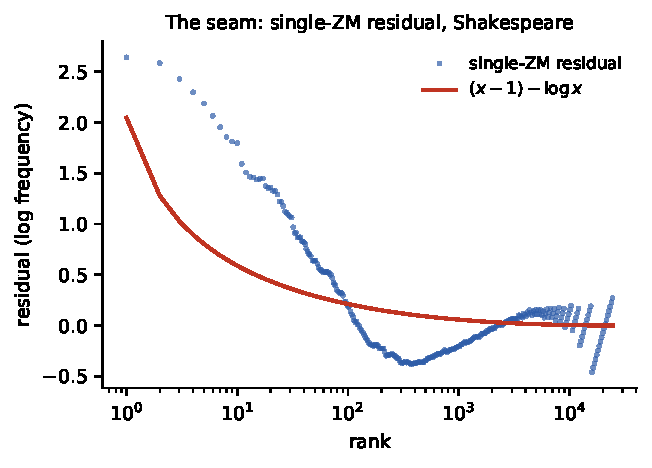
\includegraphics[width=0.72\linewidth]{fig1_residual}
\caption{The lexical seam: single-ZM residual on Shakespeare with the step-2 correction overlaid.}\end{figure}
That single-ZM fits leave structured residuals is documented: Montemurro (2001) showed the law describes only a restricted rank range, and Piantadosi (2014) exhibited the systematic error pattern directly. What has been missing is a \emph{diagnosis} --- a quantitative statement of what the structure is. Across all 25 English corpora the step-2 search recovers one of two convex correction expressions on the single-ZM residual --- $(x-1)-\log x$ on corpora with large fitted c, $e^{x-1}-x$ on the remainder --- with both expressions present in every corpus's beam, and the full enriched search improving on single ZM on 25/25 corpora (3.70--25.29\%, mean 11.02\%). These facts reproduce exactly under an independent reimplementation.

Three experiments then demonstrate that the \emph{identity} of the winning expression is a property of the scoring functional rather than of the corpus:

\begin{itemize}
\item \textbf{Free amplitude.} The canonical protocol compares corrections at unit
amplitude. Granting each candidate a fitted amplitude changes the winner on
14/25 corpora (the exponential form then wins zero). The fitted amplitude of
$(x-1)-\log x$ clusters at 0.72--0.97 on all 11 large-c corpora and near zero
elsewhere --- explaining, in one stroke, the previously puzzling fact that the
unit-amplitude correction ``helped'' on only 12/25 corpora: it helped precisely
where its natural amplitude was near one.
\item \textbf{Weighted objectives.} Under rank-weighted or frequency-weighted ZM fitting,
the winner flips from $(x-1)-\log x$ to $e^{x-1}-x$ on all 11 large-c corpora.
(This \emph{refutes} the robustness claim of our earlier draft, which was based on a
bundle that had not actually re-run the comparison.)
\item \textbf{Head-weighted scoring.} Restricting scoring to the top 100 ranks selects
$x^{x}-\sqrt{x}$ on 20/25 corpora, as anticipated by the near-collinear head-function
span identified in the April phase (17/17 span $R^2$ > 0.975 under a widened
operator grammar).
\end{itemize}
One algebraic identity dissolves much of the apparent exoticism: in the normalized coordinate, $e^{x-1} = e^{-0.95}\,r^{0.95/\ln V}$ --- the ``exponential correction'' is exactly a shallow second power law in rank. The symbolic search, whatever scoring lens it is given, keeps pointing at the same underlying object: a second component in the frequency structure. We therefore treat the residual --- the seam --- as the finding, and expression identity as a diagnostic label conditioned on the objective.

\subsection{Identity evidence: where the seam comes from}
\textbf{Ablations.} Fitting ZM to the top-100 words alone yields a clean fit (c = 5.3, RMSE 0.044) with no helpful correction; the remaining vocabulary alone likewise supports no helpful correction; the residual appears only when one curve spans both populations. (\S3.6 sharpens ``population'' beyond its historical gloss as ``function words''.)

\textbf{Negative controls.} The city-population distribution (33,535 cities, c = 100.4) yields no improving correction (composite RMSE 0.1225 vs baseline 0.1206). The US surname distribution --- a second, larger non-linguistic Zipfian system --- likewise shows no seam diagnostic (unit-amplitude correction does not help; single-ZM RMSE 0.031, an order of magnitude below any language corpus). The pattern is language-specific.

\textbf{Synthetic mixtures (deterministic protocol).} Merging two deterministic power-law populations with a small exponent gap (1.5 vs 1.3) reproduces the seam and its correction; a pure single power law fits ZM exactly (RMSE 0.0000) with no correction. Two further results refine the picture. (i) \emph{An amplitude gap suffices:} two populations with identical exponents but a tenfold scale difference still produce the seam --- the mechanism requires only separation in usage rate, not in tail exponent. (ii) \emph{Observation noise is a distinct seam source in sampled constructions:} Poisson-sampling synthetic rate populations produces additional apex curvature (cf. \S3.5 on the count floor); deterministic and sampled synthetic protocols must therefore not be mixed, and all synthetic controls in this paper are deterministic unless the observation model is the explicit object of study.

\subsection{The smooth two-regime model absorbs the seam; the width law}
\begin{figure}[t]\centering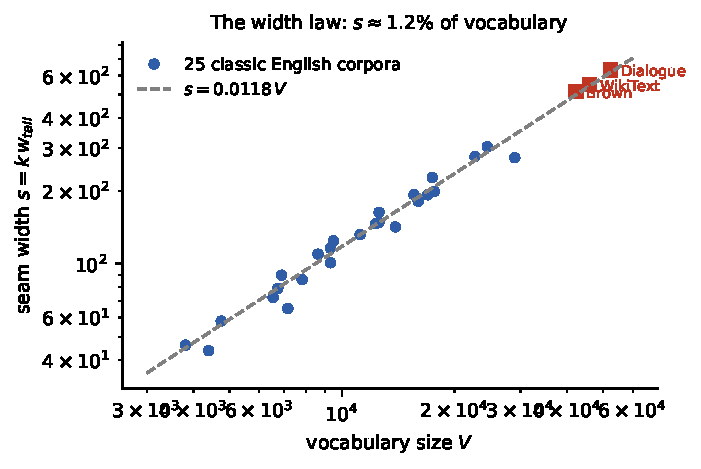
\includegraphics[width=0.72\linewidth]{fig3_s_law}
\caption{The width law: seam width $s$ against vocabulary $V$ for 25 classic corpora (circles) and three modern registers (squares), with $s=0.0118\,V$.}\end{figure}
Refitting the canonical smooth model confirms the April results: it improves on single ZM, hard-piecewise, and continuous-piecewise alternatives on 25/25 corpora, and --- the mechanistic distinction --- running the symbolic diagnostic on the residual left by each model shows the two-regime model absorbs the seam completely (helpful corrections on 0/25 corpora; median residual gain -0.002) while MOEZipf, the strongest single-regime extension, leaves it recoverable (19/25; median +0.017). On a planted two-regime mixture MOEZipf cannot absorb the constructed signal. In the gate-family comparison, erf wins BIC on 24/25 English corpora (arctan takes only Dubliners; median independent-gate BIC spread 677), and the falsification check recovers logistic on 25/25 logistic-generated synthetic corpora, never spuriously preferring erf. The MOEZipf residual, where present, takes a characteristic \emph{negative} Itakura--Saito shape --- the single-regime skew over-corrects the apex --- a sharper statement than ``structure remains''.

\textbf{The width law.} Profile likelihood shows the gate centre k is sharply identified within each corpus (median $\Delta$BIC $\le$ 2 interval $\pm$1\%) yet obeys no tight law in V ($\beta = 0.758$, CI [0.367, 1.149], $R^2$ = 0.386) --- the earlier coupled-model $k \approx \sqrt{V}$ claim is confirmed retired. The lawful quantity is one level up: the tail transition scale $s = k\,w_{tail}$ satisfies

\begin{equation}s \propto  V^{1.003},  \ \text{95\% CI}\  [0.928, 1.079],  R^2 = 0.967\end{equation}
equivalently \textbf{$s \approx 0.012\,V$}: the seam occupies a constant $\approx$1.2\% band of the vocabulary axis. Measured twice (indirectly at the k-profile optimum, and by direct s-profiling, which is sharp to better than grid resolution), the constant holds across the 25 classic corpora (0.0118), Brown (0.0122), WikiText (0.0120), and film dialogue (0.0121) --- five centuries and four registers within $\pm$3\%. (An early six-language check returned smaller interior values, 0.0068--0.0096; the cross-language analysis below shows these were sampling-depth artifacts, and that the constant is universal at matched depth.) Three initial cross-language fits that violated the law proved to be optimizer escapes (gate-width and tail-width bounds pinned simultaneously) and re-fit cleanly under tightened bounds; the surname control fits a distinct constant (0.0266), as an unrelated system should.

We emphasize what kind of object equation (3) measures. Prior two-regime accounts parameterize a crossover \emph{location} --- a fixed finite core vocabulary (Gerlach and Altmann 2013), a break at the mean constituent vocabulary (Williams et al. 2015), a crossover frequency (Montemurro 2001) --- and none assigns the transition a width. Simulation shows the width is a \emph{shared invariant} of language-like generative processes rather than a discriminator among them: running the Gerlach-Altmann model with its published English constants yields s/V = 0.0112--0.0125 across V = 16k--88k, and a one-class variant with no core at all yields 0.0118 --- the real-language value to three decimals. The constant is nonetheless family-specific, not an artifact of the fitting operator: constant-innovation (single-regime) growth fits a distinct stable constant (0.0101), and the surname system another (0.0266). The empirical content of equation (3) for language is therefore threefold: the width exists as a measurable object; it is invariant across registers, centuries, sizes, and compositions at 0.0118; and its value sits precisely on the decaying-innovation family's fingerprint. What discriminates between mechanistic accounts is not the width but the boundary's identity (\S3.6) and its depth behaviour (\S3.4).

\textbf{Composition robustness.} Williams et al. (2015) argue that two-regime structure in rank-frequency curves is an artifact of aggregating texts, with a mixing-induced break at rank $\approx$ N\_avg, the mean per-constituent vocabulary --- and that even single texts break only insofar as they are internally mixed. The width law provides a direct test, and it fails to confirm the mixing account twice. First, splitting the 25-corpus panel by composition --- 15 single continuous works against 10 collections (Shakespeare's 37 plays, the Bible's 66 books, Aesop's hundreds of fables) --- yields statistically indistinguishable width constants: mean s/V 0.0119 vs 0.0113 (Welch p = 0.19; bootstrap CI on the difference [-0.0015, +0.0002]), with the two groups fully interleaved and the insignificant trend pointing \emph{opposite} to mixing-inflation. Second, a forced- mixing experiment (f12) concatenates 14 single-author works into mixtures of m = 2, 4, 7, and 14 under one identical fitter: if mixing drove the seam, the fitted transition should migrate toward N\_avg (\~{}10$^{4}$) and its width law should break with m. Neither happens. Median s/V by mixing degree is 0.0119, 0.0127, 0.0128, 0.0123, 0.0120 for m = 1, 2, 4, 7, 14 --- no trend across a fourteen-fold change in aggregation --- and the seam centre stays one to two orders of magnitude below N\_avg at every m (median k/N\_avg 0.021 at m = 1, 0.079 at m = 14, its mild growth tracking V rather than N\_avg). Pooled over all 27 fits, s $\propto$ $V^{0.977}$ with $R^2$ = 0.983 --- forced aggregation adds points \emph{on} the width law's line. Whatever text mixing does to the deep tail it studies, it neither creates nor moves the seam: the two objects live at different ranks, and only theirs is composition-relative.

\textbf{Cross-language depth unification.} A 33-corpus multilingual extension (four deep corpora fit at full depth plus a 29-corpus panel spanning eleven languages fetched from Project Gutenberg) resolves the cross-language question: the width fraction correlates with per-type sampling depth (tokens-per-type) at r = +0.94, deep corpora (tokens/type $\ge$ 12) sit at median s/V = 0.0111 against English's 0.0118 at its greater depths, and the apparently ``low'' languages (Hungarian 0.0076, Finnish 0.0079) are precisely the morphologically rich ones whose token mass spreads over 2--3$\times$ more types, leaving each type under-sampled. The earlier shallow interior values (0.0068--0.0096) were depth artifacts. Two follow-ups close the case. First, within-corpus depth slicing (binomial thinning, the \S3.4 protocol): sliced to matched per-type depths, English, French, Spanish, and Russian ride a single rising curve in (tokens-per-type, s/V) space --- pooled correlation +0.93, within-depth cross-language agreement to $\pm$0.0005, mean within-bin spread 0.37 of the total spread --- with detectable optimizer escapes (7/54 fits, all bound-pinned) excluded. Second, within-language concatenation to matched depth (a valid depth amplifier by the composition result above): the five languages reaching tokens-per-type $\ge$ 15 land at median s/V = 0.0122 against English's 0.0118, while the morphologically rich languages that cannot yet reach depth sit on the approach curve at their accessible depths (one flagged exception: the deep Spanish concatenation runs high, 0.0149, plausibly its four-century era mixture). The reading is a single universal depth function, still rising slowly at the greatest depths probed (tokens-per-type $\approx$ 30--40), whose value over the depth range typical of single-work corpora is the $\approx$1.2\% constant of equation (3) --- the width is governed by the same sampling-depth dial that \S3.4 establishes for c, unifying the two sections under one mechanism.

\textbf{Instrument calibration.} Because the width is the paper's headline quantity, the estimator was calibrated against ground truth by parametric bootstrap: taking each corpus's fitted model as the generating truth, Poisson- resampling its token counts, and refitting (75 refits). Recovery ratio s\_hat/s\_true: median 1.032, IQR [1.006, 1.062], with 21/25 corpora within [0.8, 1.25]; the exceptions are optimizer escapes to bound-pinned basins --- a detectable failure mode, screened in the empirical pipeline by the profile-likelihood cross-checks of \S3.3. A model-light envelope measurement (head-window and tail-window ZM extrapolations; the transition as the zone neither explains, over an 18-setting sensitivity grid) gives directional confirmation that the transition is a property of the curve rather than the fitter --- language's zone is wider than that of matched single-regime multinomial twins on 16/25 corpora (median excess +0.011) --- with the caveat that model-free width estimation is low-powered, partly because ranking a sample induces order-statistics structure even under a true single law. A first planted-seam calibration attempt using an out-of-regime synthetic grid failed and is preserved in the repository as a documented negative.

\subsection{Mandelbrot's c is sampling depth}
\begin{figure}[t]\centering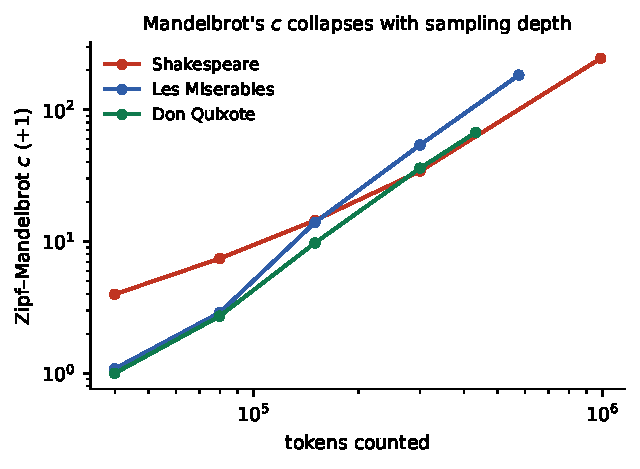
\includegraphics[width=0.72\linewidth]{fig2_c_collapse}
\caption{Subsampling collapses the fitted shift $c$ along smooth trajectories.}\end{figure}
Slicing any corpus to smaller token counts collapses its fitted c along a smooth trajectory: Shakespeare's complete works fall from c = 244 (989k tokens) through 33, 13, and 6 to c = 3 at 40k tokens; Les Misérables from 182 to 0.1; Don Quixote from 66 to 0. Binomial thinning of the full count vector reproduces the prefix-slice trajectories closely, establishing the collapse as pure sampling statistics rather than textual nonstationarity. The King James Bible --- an anthology of 66 books --- resists collapse longest (171 $\to$ 18), consistent with aggregate structure.

The step-2 winner flips along the same axis on 6/6 corpora tested, following one ladder --- $(x-1)-\log x$ at depth, $e^{x-1}-x$ in the mid range, $x^{x}-\sqrt{x}$ when shallow --- so the ``three corpus regimes'' of the earlier draft (and of our multilingual comparison) are one phenomenon at three sampling depths. A simple classifier predicts the winner label from (log tokens, hapax share, type--token ratio) with 80\% leave-one-out accuracy and no curve fitting at all.

Size-dependence of Zipfian fits is itself documented: Bernhardsson et al. (2009) proposed text-length-dependent distribution parameters, and Font-Clos et al. (2013) argued the apparent drift of the Zipf exponent with length is an artifact of the growing weight of a second frequency regime under a scale-invariant shape. The c(T) trajectories give that discussion a parametric handle on the standard ZM form: c is the parameter that absorbs depth, b is comparatively stable, and cross-corpus c comparisons are meaningful only depth-matched. At the opposite extreme of parameter space, Mačutek (2022) showed that ZM fits can ``explode'' (b, c $\to$ $\infty$ jointly, converging to a geometric distribution) on grapheme-like data --- a second, independent sense in which raw ZM parameter values are estimation artifacts unless their regime is identified.

\textbf{The matched-size panel.} Re-measuring 21 corpora at an identical 65k-token depth dissolves most of the previously reported cross-language c contrast: English classics drop to c $\in$ [0, 24] (median 6.3) while other languages sit at c $\approx$ 0 (median 0.00, max 0.71). The residual difference is genuine and is isolated by a natural experiment: \emph{War and Peace} at 65k tokens carries c = 10.1 in English translation and c = 0.0 in the Russian original --- same text, same author, same depth; the difference is what the language's morphology does to word frequencies. All cross-corpus statements about c in this paper are therefore depth-annotated, and we flag the same requirement for the prior literature.

\subsection{A generative account: from histogram to curve, and across sizes}
\begin{figure}[t]\centering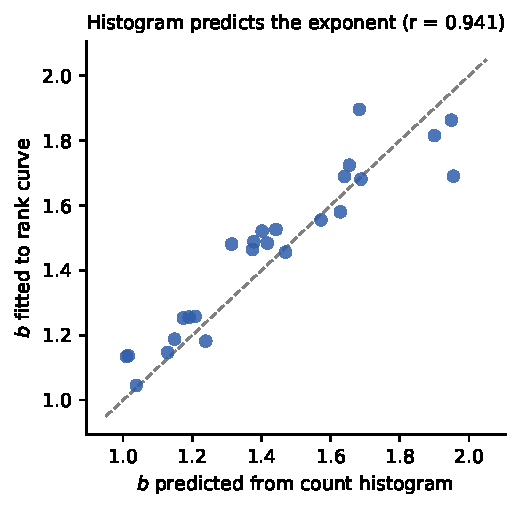
\includegraphics[width=0.5\linewidth]{fig4_b_prediction}
\caption{The exponent predicted from the count histogram alone versus the exponent fitted to the rank curve (25 corpora).}\end{figure}
\begin{figure}[t]\centering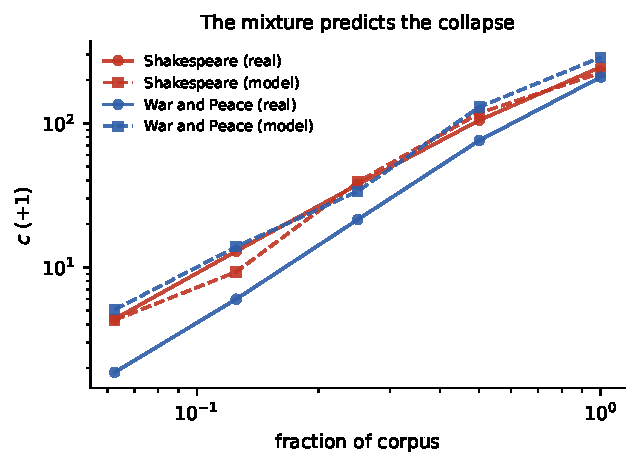
\includegraphics[width=0.72\linewidth]{fig5_trajectories}
\caption{Downward $c(T)$ trajectories: binomially thinned data (circles) versus the mixture fitted at full depth (squares).}\end{figure}
\begin{figure}[t]\centering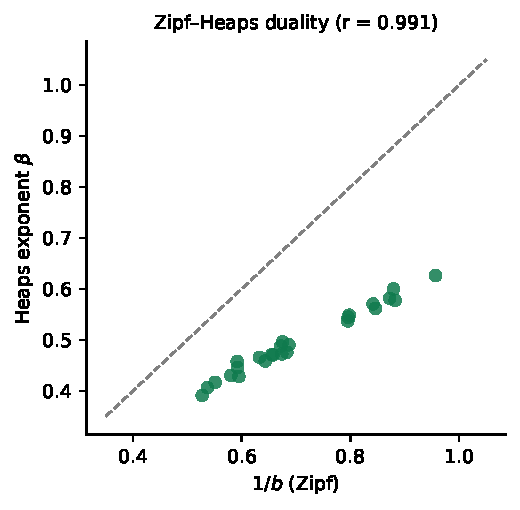
\includegraphics[width=0.5\linewidth]{fig6_heaps}
\caption{Heaps' exponent against $1/b$: the measured Zipf--Heaps duality (r = 0.991).}\end{figure}
\textbf{At fitted depth.} The five-parameter zero-truncated Poisson--lognormal mixture estimated from a corpus's unordered count histogram --- never seeing ranks --- regenerates the corpus's fitted ZM parameters when pushed through the observation model: across 25 corpora, predicted b correlates with actual at r = 0.941 with median absolute error $\approx$4\% (\emph{War and Peace} 1.688 predicted vs 1.681 actual; \emph{Ulysses} 1.038 vs 1.045), and predicted c is on the correct scale (corr on log(1+c) = 0.82). A theoretically instructive negative: the same prediction computed from the \emph{latent} quantile curve, ignoring the count floor, fails catastrophically (b $\approx$ 8--12) --- \textbf{the impossibility of observing a count below one is load-bearing for the observable shape of Zipf's law.} The once-words are not a nuisance at the tail; they are structural.

\textbf{Across sizes.} Fitted at full depth, the mixture now reproduces the entire downward c(T) collapse (Shakespeare: model 223/116/38/8.3/3.3 against real 245/104/36/12/3.4) and matches vocabulary-growth curves V(T) to 1--2\% at every scale. Fitted only to a 150k-token fragment and simulated forward at full scale --- genuine out-of-sample extrapolation, up to 6.6$\times$ --- it predicts:

\begin{center}\small\begin{tabular}{llll}\toprule
corpus (extrapolation) & V pred $\to$ real & b pred $\to$ real & c pred $\to$ real \\ \midrule
Shakespeare (6.6$\times$) & 24,072 $\to$ 24,458 & 1.725 $\to$ 1.724 & 262 $\to$ 245 \\
War and Peace (3.9$\times$) & 17,183 $\to$ 17,445 & 1.685 $\to$ 1.680 & 209.5 $\to$ 208.1 \\
Les Misérables (3.8$\times$) & 21,844 $\to$ 22,677 & 1.538 $\to$ 1.527 & 250 $\to$ 184 \\
Moby Dick (1.5$\times$) & 16,970 $\to$ 16,956 & 1.190 $\to$ 1.182 & 18.6 $\to$ 10.7 \\
\bottomrule\end{tabular}\end{center}
Vocabulary is predicted to \~{}2\% and the exponent to \~{}0.3\%; the shift is predicted to first approximation (0.7\%--36\% depending on corpus and tail variant; a heavy lower tail helps on some corpora and not others, and neither tail family dominates).

Extrapolating lexical statistics across sizes is an established program: LNRE models (Baayen 2001), implemented in zipfR (Evert and Baroni 2007), extrapolate vocabulary size and frequency spectra to larger samples, and our binomial-thinning check is the same interpolation mathematics. What the mixture adds to that program is the \emph{rank law itself}: the extrapolation target here is the fitted ZM parameter vector (b, c) and its full depth trajectory, an object LNRE extrapolation does not address. Because V(T) is predicted, Heaps' law also comes with the account. The reciprocal relation between Heaps' and Zipf's exponents ($\beta \approx 1/b$) is a known theoretical result, derived by several authors in the infinite-size limit (see Font-Clos et al. 2013 and references therein); on our panel the measured Heaps exponent (median $\beta = 0.476$, range 0.39--0.63) confirms it at finite sizes with $\mathrm{corr}(\beta, 1/b)$ = 0.991, and in the generative account both exponents emerge jointly from one fitted mixture rather than being related after the fact.

\textbf{The mixture contains the width law.} A final test closes the loop between this section and \S3.3: simulating each corpus from its fitted mixture and fitting the same nine-parameter gate model to the synthetic curves reproduces the measured seam width almost exactly on 16/25 corpora at the maximum-likelihood solution (median ratio 1.02), with the failures confined to deeply-sampled corpora whose ML fit lands in a blurred-head likelihood basin. Reselecting those corpora's basins by an independent criterion --- cross-size prediction error under thinning, which never sees rank curves or widths --- heals 8 of the 9 failures to ratios 0.94--1.03 (median 1.01; one corpus, \emph{Critique of Pure Reason}, resists), from basins statistically indistinguishable in likelihood ($\Delta$NLL 0--11). The width law of equation (3) is therefore generated by the mixture-plus-count-floor account at the physical basin, and two independent observables --- cross-size prediction and seam width --- converge on which basin that is. Notably, the healed basins differ widely in latent parameters: the width is an invariant of basins consistent with the histogram \emph{and its thinned versions}, not a readout of any latent quantity --- the depth dimension is load-bearing here exactly as in \S3.4.

\textbf{Identifiability, stated plainly.} The latent mixture is only weakly identified from a single depth: solutions differing in $\sigma_T$ by a factor two and in implied total (unseen-inclusive) type count by a factor thirty fit one histogram within $\Delta$NLL $\le$ 5, and the maximum-likelihood solution is frequently \emph{not} the best cross-size predictor. All claims in this section are therefore claims about predicted observables; we make no claims about latent parameter values, and two earlier candidate claims of exactly that kind are retired in \S4.2. Under broad-basin fitting, the count histogram alone statistically demands a second component only in the largest corpora (3/10 by BIC); the two-population structure rests on the identity- and structure-aware evidence of \S\S3.2--3.4 and 3.6, not on histogram mixture selection.

\subsection{The seam is a usage boundary, not the grammatical one}
With reliable word-level labels (\S2.6), we can finally ask \emph{what} the two populations are. The labeled instantaneous closed-class share at rank r declines through 50\% at rank $k_{POS}$; the statistical gate centre sits a \textbf{median factor 3.10 deeper} (per-corpus correlation between the two positions is weak, r $\approx$ 0.20, and gate widths do not track labeled transition widths). The statistical high-usage club is therefore \emph{not} the closed class: it comprises the grammatical core plus the most frequent content words --- items that behave statistically like function words without being them. The seam is drawn by usage dynamics, roughly three times deeper into the vocabulary than the grammar textbook's boundary. This finding is consistent with the ablation evidence (which manipulated the statistical club), with the amplitude-gap sufficiency result of \S3.2, and with the annotation data itself; it retires the strong identification ``seam = function/content boundary'' and, with it, any equation of the statistical transition centre with the POS crossover. On the labeled subsample the POS crossover scaling is also weaker ($\beta = 0.298$, CI [0.08, 0.52], n = 10) than the tagger-based estimate of earlier drafts (0.545), which we now report only with that caveat. As a byproduct, the transfer property of the high-c head shape strengthens: a degree-5 head-shape correction fitted on \emph{War and Peace} transfers to the King James Bible at essentially in-domain accuracy (0.1498 vs 0.1494; ZM baseline 0.1882).

\subsection{$\lambda$-ZM: a practical formula}
Equation (2) --- ZM plus one term with one amplitude --- is preferred by BIC over both single ZM and MOEZipf (each fitted at its best, including MOEZipf by direct least squares on the shared objective) on \textbf{25/25 English corpora}, with median RMSE improvement 10.2\% (range 2.6--23.0\%) --- comparable to the terminal ten-step symbolic search from a closed-form expression. On the extended panel it wins BIC on 10/10 further corpora (Brown +14.1\%, WikiText +9.9\%, dialogue +5.8\%; six additional languages +9.0--22.5\%), and on the seven canonical non-English corpora it improves fit by 6.4--21.6\% including the c $\approx$ 0 scripts (Mandarin +21.6\%, Arabic +14.3\%, Russian +12.9\%). Lifetime record across every corpus tested in this project: 42/42. Interpretation is built in: by the identity of \S3.1 the added term is a second shallow power-law component --- $\lambda$-ZM is the two-population structure in its minimal parametric form. (On the surname control, $\lambda$-ZM also improves fit --- as any extra parameter polishes an already near-perfect curve --- while the parameter-free seam diagnostic correctly stays silent; the diagnostic, not the formula, carries the specificity claim.)

\section{Discussion}
\subsection{What this work shows}
(a) The single-ZM residual is a reproducible, low-dimensional structure --- the lexical seam --- whose symbolic label is scoring-conditioned but whose existence, localization, and absorption behaviour are invariant across two independent implementations, three scoring families, and 42 corpora.

(b) The seam separates a small high-usage vocabulary from the broad lexicon; it requires only a usage-rate gap between populations; it is absent from non-linguistic Zipfian systems; and its rank-space width is a constant $\approx$1.2\% of vocabulary --- across registers and centuries of English, across forced changes of corpus composition, and across twelve languages once per-type sampling depth is matched, with the estimator calibrated against planted ground truth. The width is, to our knowledge, a new empirical object --- prior two-regime accounts parameterize only a crossover location --- and its proportional scaling with V is a regularity that simulation shows every language-like growth account tested in fact obeys (\S3.3): a shared invariant with a family-specific constant, on whose decaying-innovation value natural language sits.

(c) Mandelbrot's c is a sampling-depth dial, not a stylistic constant: its value, its collapse under subsampling, and the accompanying ladder of symbolic labels are predicted by the generative account; cross-language c comparisons require matched depth, where a small, genuinely morphological residual remains (the translation-pair experiment).

(d) A five-parameter mixture pushed through the Poisson observation model with its count floor regenerates the law's parameters from the histogram, predicts a full corpus from a fragment, reproduces the seam width of equation (3) on 24/25 corpora at the prediction-selected basin, and carries Heaps' law as its dual. The observable predictions are robust across mixture basins; latent parameters are not identified and are not claimed.

(e) The seam is a usage boundary lying \~{}3$\times$ deeper than the closed-class crossover --- the two-population structure of language is drawn by usage dynamics, not by grammatical category.

(f) $\lambda$-ZM offers the practical upgrade: one added term, undefeated in fair comparisons across 13 languages.

\subsection{Retired claims: the ledger}
Each of the following was, at some stage of this project, a stated finding. Each was retired by an experiment we ran on ourselves. We report them because the final claim set is defined as much by what survived as by what did not.

\begin{enumerate}
\item \textbf{$k \approx \sqrt{V}$ scaling of the transition centre} --- an artifact of the coupled
single-width parameterization; under the decoupled model k is identified per
corpus but obeys no tight law (the law lives in s, eq. 3).
\item \textbf{``WLS does not alter winner identity''} (v5.1 \S3.1) --- refuted; all 11
large-c corpora flip under weighted objectives (\S3.1).
\item \textbf{A universal content-population dispersion ($\sigma_T$ $\approx$ 1.6)} --- an artifact of a
restricted optimization basin; the latent dispersion is not identified from
single-depth data ($\Delta$NLL $\le$ 5 solutions span $\sigma_T$ 1.9--4.0).
\item \textbf{A cross-language ``morphology dial'' in $\sigma_T$} --- the model-free check reverses
the ordering (r = -0.53); the fitted gradient tracked tokens-per-type at the
chosen depth.
\item \textbf{``Two components demanded by the histogram on 25/25 corpora''} --- a
narrow-basin artifact; under broad-basin fitting the histogram alone demands
two components on only the largest corpora (3/10). The two-population case
rests on identity/structure evidence.
\item \textbf{Seam = function/content boundary} --- retired by direct annotation
comparison (\S3.6); the seam is a usage boundary \~{}3$\times$ deeper.
\item \textbf{A $\sqrt{e}$ width-prediction constant} --- a four-decimal numerical coincidence
that died with the estimator that produced it.
\item \textbf{The convex-conjugation relation between the two correction generators}
(v5.1 \S3.1) --- removed as incorrect following external audit; with it, all
``curved probability manifold'' language, replaced throughout by
scoring-conditioned statements about a near-collinear head-function span.
\end{enumerate}
\subsection{Relation to prior work}
\emph{Two regimes.} The observation that one ZM curve does not span the lexicon, and the hypothesis that two lexical populations underlie it, date to Ferrer-i-Cancho and Solé (2001) and Montemurro (2001), who documented dual scaling regimes and proposed, respectively, a kernel/unlimited lexicon split and a Tsallis-form generalization. We contribute the seam's localization by word identity, its absorption test, its width --- a measured object where prior accounts have only a crossover location --- its depth-dependence, and its annotation-based reinterpretation as a usage boundary.

\emph{Generative two-class models.} Gerlach and Altmann (2013) is the closest prior framework: a stochastic vocabulary-growth model with a finite set of core words and an unbounded non-core class that generalizes both Zipf's and Heaps' laws to two scaling regimes and fits databases spanning eight orders of magnitude with language-level parameters. The width law is a measurement their program did not make --- and, strikingly, simulating their model with their published constants shows it \emph{obeys} equation (3) (s/V $\approx$ 0.0122 across V = 16k--88k), as does a coreless one-class variant (0.0118): the width is insensitive to exactly the structure that distinguishes their account, while remaining a fingerprint of the decaying-innovation growth family (\S3.3). The width law is thus an invariant that any adequate account inherits rather than a test that separates them; what separates accounts empirically is the boundary's identity against labeled word classes (\S3.6, which their framework does not address) and the depth trajectory of the fitted parameters (\S3.4). Their model also operates in frequency-distribution space without a residual diagnostic or a transition-width object.

\emph{Text mixing.} Williams et al. (2015) counter the core/non-core reading with the hypothesis that scaling breaks are artifacts of aggregating texts, breaking at the mean constituent vocabulary N\_avg. Their break and our seam are different objects at different scales (N\_avg \~{} 10$^{4}$ vs k \~{} 10$^{2}$--10$^{3}$), and \S3.3's two composition tests --- the single-vs-aggregate split and the forced-mixing experiment --- show the seam and its width law are indifferent to composition, which the mixing account does not predict for a mixing-derived feature.

\emph{Single-regime extensions.} MOEZipf (Pérez-Casany and Casellas 2013) remains the strongest single-regime extension and our principal comparison; the residual-absorption asymmetry (0/25 vs 19/25) and the sign of its leftover residual are, we believe, new characterizations.

\emph{Population models and extrapolation.} Lognormal population models date to Carroll (1967), and mixture accounts of word-frequency spectra --- including the observation that entrenched vocabulary is approximately lognormal --- underpin the LNRE program (Baayen 2001; Evert and Baroni 2007), whose central application is extrapolating vocabulary and spectra across sample sizes. Our contribution is to make a two-component lognormal account predictive \emph{of the rank law}: the zero-truncated Poisson observation model --- including the demonstration that the count floor is what reconciles lognormal populations with power-law-looking observables --- carries the histogram to the fitted ZM parameters and their depth trajectories, with identifiability limits stated precisely. The Zipf--Heaps exponent duality $\beta \approx 1/b$ is likewise a known derivation (references in Font-Clos et al. 2013); our panel supplies its finite-size empirical confirmation and its joint emergence from one fitted mixture. Size-dependence of fitted parameters connects to Bernhardsson et al. (2009) and Font-Clos et al. (2013), and the estimation-fragility of raw ZM parameter values to Mačutek (2022), as discussed in \S3.4.

\emph{Method.} The symbolic-regression literature (Schmidt and Lipson 2009; Udrescu and Tegmark 2020; Cranmer 2023) supplies the diagnostic instrument; we found no prior application of symbolic regression to word-frequency laws or their residuals. Using enumerative SR as a \emph{residual auditor} for a classical law --- and then auditing the auditor's own labels --- is, to our knowledge, novel methodologically.

\subsection{Preliminary observations in neural language models}
Two exploratory experiments (repository, L-series) suggest the seam is visible inside models trained on language: GPT-2's input-embedding norm curve is decisively two-regime in token rank ($\Delta$BIC 55.8, with a sharp break at the ultra-frequent token club), and a 23M-parameter model trained from scratch shows a seam-shaped per-rank loss curve at every checkpoint whose position migrates with training-token budget --- from the head club (ranks $\approx$ 12$\to$35 over the first 2M tokens) into the deep vocabulary ($\approx$15k--23k after 8M) --- a learning-frontier analogue of the sampling-depth ladder. A theoretical bridge exists: Dębowski (2026) derives neural scaling laws from Zipf's law through Heaps' law and Hilberg's hypothesis, making the statistics studied here directly relevant to model-scaling questions. These single-run observations are reported as motivation for separate work, not as claims of this paper.

\subsection{Limitations}
The English core sample is Gutenberg literary text; the register panel is small (three modern corpora) and the non-English corpora are single works at modest depths, with tokenization caveats (jieba's single-character bias for Mandarin; translation-year dating for diachronic checks, which showed no signal). BIC comparisons ignore word-level autocorrelation. Annotation covers ten corpora (\~{}17k types) with a single-corpus inter-annotator pilot. The latent mixture's identifiability limits are stated in \S3.5 and bound every generative claim; the extrapolation experiments cover four corpora and one direction of protocol (binomial fragments). The cross-language width panel spans eleven languages but tops out near tokens-per-type $\approx$ 19; the deepest sampling regimes (tokens/type > 25) remain unprobed outside English, and whitespace-unsegmented scripts (Mandarin, Arabic) are excluded throughout. The PMF/likelihood-space program of earlier drafts (Seam-Mandelbrot PMF, soft-k regularization, per-book anthology decomposition) is out of scope here and held for a companion paper, as is the neural-model line of \S4.4.

\section{Conclusion}
A single structure --- a seam between a small high-usage vocabulary and the broad lexicon, drawn by usage rather than grammar --- accounts for the systematic residual of the Zipf--Mandelbrot law, fixes its formula with one term, explains its mysterious shift parameter as sampling depth, sets a new invariant (a transition width of $\approx$1.2\% of vocabulary, universal across twelve languages at matched sampling depth and measured by a ground-truth-calibrated estimator), and supports a generative model that predicts a corpus's rank law, vocabulary growth, and Heaps exponent from a fragment of its text. The claims survived two independent implementations, an external adversarial audit, falsification-checked model comparisons, and eight self-inflicted retirements. What began as a curiosity in a fit's error term ends as a measurement of how language allocates its words.

\section{Acknowledgments}
The author thanks Claude (Anthropic) for extensive assistance with experiment design, implementation, analysis, and drafting throughout this project. All claims trace to reproducible artifacts in the public repository.

\section{Code and data availability}
All code, corpus-processing pipelines, per-experiment outputs, and the claim-to-CSV provenance map are public at https://github.com/Surebob/lexical-seam-paper --- every quantitative claim in this paper maps to a versioned CSV there (docs/MANUSCRIPT\_v6\_CLAIM\_MAP.md). Large third-party corpora (Brown, WikiText-103, film dialogue, the surname census) are fetched by included scripts rather than redistributed.

\section*{References}
Baayen RH. 2001. \emph{Word Frequency Distributions.} Kluwer Academic Publishers.

Bernhardsson S, da Rocha LEC, Minnhagen P. 2009. The meta book and size-dependent properties of written language. \emph{New Journal of Physics} 11:123015.

Carroll JB. 1967. On sampling from a lognormal model of word-frequency distribution. In \emph{Computational Analysis of Present-Day American English}.

Cranmer M. 2023. Interpretable machine learning for science with PySR. \emph{arXiv:2305.01582.}

Dębowski Ł. 2026. From Zipf's law to neural scaling through Heaps' law and Hilberg's hypothesis. \emph{arXiv:2512.13491.}

Evert S, Baroni M. 2007. zipfR: word frequency distributions in R. In \emph{Proceedings of the 45th Annual Meeting of the ACL, Demo Session}, 29--32.

Ferrer-i-Cancho R, Solé RV. 2001. Two regimes in the frequency of words and the origins of complex lexicons. \emph{Journal of Quantitative Linguistics} 8(3):165--173.

Font-Clos F, Boleda G, Corral Á. 2013. A scaling law beyond Zipf's law and its relation to Heaps' law. \emph{New Journal of Physics} 15:093033.

Gerlach M, Altmann EG. 2013. Stochastic model for the vocabulary growth in natural languages. \emph{Physical Review X} 3:021006.

Mačutek J. 2022. Why do parameter values in the Zipf-Mandelbrot distribution sometimes explode? \emph{Journal of Quantitative Linguistics} 29(4). doi: 10.1080/09296174.2021.1887613.

Mandelbrot B. 1953. An informational theory of the statistical structure of language. In \emph{Communication Theory}, ed. W. Jackson. Butterworth.

Montemurro MA. 2001. Beyond the Zipf--Mandelbrot law in quantitative linguistics. \emph{Physica A} 300(3--4):567--578.

Pérez-Casany M, Casellas A. 2013. Marshall-Olkin Extended Zipf distribution. \emph{arXiv:1304.4540.}

Piantadosi ST. 2014. Zipf's word frequency law in natural language: a critical review and future directions. \emph{Psychonomic Bulletin \& Review} 21:1112--1130.

Schmidt M, Lipson H. 2009. Distilling free-form natural laws from experimental data. \emph{Science} 324:81--85.

Udrescu SM, Tegmark M. 2020. AI Feynman. \emph{Science Advances} 6(16).

Williams JR, Bagrow JP, Danforth CM, Dodds PS. 2015. Text mixing shapes the anatomy of rank-frequency distributions. \emph{Physical Review E} 91:052811.

Zipf GK. 1949. \emph{Human Behavior and the Principle of Least Effort.} Addison-Wesley.

\section*{Appendix A: claim provenance (summary)}
Every number above traces to a canonical CSV in the repository. Key mappings --- \S3.1: \texttt{experiments/1a\_*/outputs}, \texttt{f1\_fresh\_reproduction}, \texttt{f9\_legacy\_reruns} (WLS), \texttt{f3} (head-weighted); \S3.2: \texttt{2a}, \texttt{1b}, \texttt{f5a} (surnames), \texttt{f11} (2b deterministic); \S3.3: \texttt{2c}, \texttt{3e}, \texttt{f2\_k\_profile\_likelihood}, \texttt{f2b\_s\_profile}, \texttt{f5b}/\texttt{f5c}, \texttt{f12\_forced\_mixing} (composition); \S3.4: \texttt{f6\_c\_sampling\_depth}, \texttt{f8\_matched\_size\_panel}, \texttt{f11} (classifier); \S3.5: \texttt{f4d}, \texttt{f7\_histogram\_predicts\_curve}, \texttt{f6b\_heavy\_tail\_ extrapolation}, \texttt{f4f}/\texttt{f4g} (identifiability), \texttt{f11} (Heaps); \S3.6: \texttt{f10\_gate\_vs\_labels}, \texttt{data/annotations}, \texttt{f9} (transfers); \S3.7: \texttt{f1}, \texttt{f3}, \texttt{f5a}. Retired-claim experiments: \S4.2 items map to \texttt{f2}, \texttt{f9}, \texttt{f4f}, \texttt{f4f}, \texttt{f4g}, \texttt{f10}, \texttt{f4d}+\texttt{f4f}, and the 2026-04 external audit respectively. A full v6 claim-to-CSV map will be regenerated before submission.

\end{document}